\section*{Methods}
This section outlines the methodology for creating the CholecInstanceSeg dataset, divided into four main topics: data sources, labelling protocol, annotation tool and techniques, and the annotation workflow and procedures.

First, we describe the data sources and how the frames were extracted. Next, we outline the principles guiding our instance segmentation dataset, emphasizing the labelling protocol. We then discuss the tools and techniques used to overcome annotation challenges. Finally, we provide a detailed account of the annotation process, including information about the annotators and the time spent on creating CholecInstanceSeg.

\subsection*{Data Sources}
The CholecInstanceSeg dataset is curated using frames extracted from three existing laparoscopic cholecystectomy datasets: Cholec80 \cite{endonet_cis}, CholecT50 \cite{NWOYE2022102433_rendevous_cis}, and CholecSeg8k \cite{cholecseg8k_cis}, containing a total of 85 image sequences. 
These datasets are publicly available subsets of the in-house Cholec120 dataset \cite{twinanda2018rsdnet_cis} from the CAMMA research group \robustrevref{1}{7}\revnew{which was recorded at the University Hospital of Strasbourg \cite{endonet_cis,NWOYE2022102433_rendevous_cis}} 
. The interrelation between these datasets is illustrated in  \figref{fig:cholec_dataset_relationships}. 

When discussing the source datasets, we distinguish between videos and image sequences. Videos are multimedia compressed files provided in formats such as .mp4, while image sequences refer to extracted sequential frames from videos. 

\robustrevref{1}{5}\revnew{The frames from Cholec80 and CholecT50 used in CholecInstanceSeg are primarily at a resolution of 854x480 pixels, consistent with the original Cholec80 and CholecT50 datasets. However, three sequences from CholecT50 are provided at a higher resolution of 1920x1080 pixels. CholecT50 contains pre-extracted image sequences and we used these as is, while frames from Cholec80 were extracted at 1 fps using the FFMPEG library.}

CholecInstanceSeg includes frames from publicly available datasets that already have the necessary consents and ethical considerations. Additionally, the licenses for the source datasets permit the enhancement of the data with further annotations (\href{https://github.com/CAMMA-public/TF-Cholec80}{Cholec80 license}, \href{https://github.com/CAMMA-public/cholect50}{CholecT50 license}, \href{https://www.kaggle.com/datasets/newslab/cholecseg8k_cis}{CholecSeg8k license}).

\begin{figure}[ht]
\centering
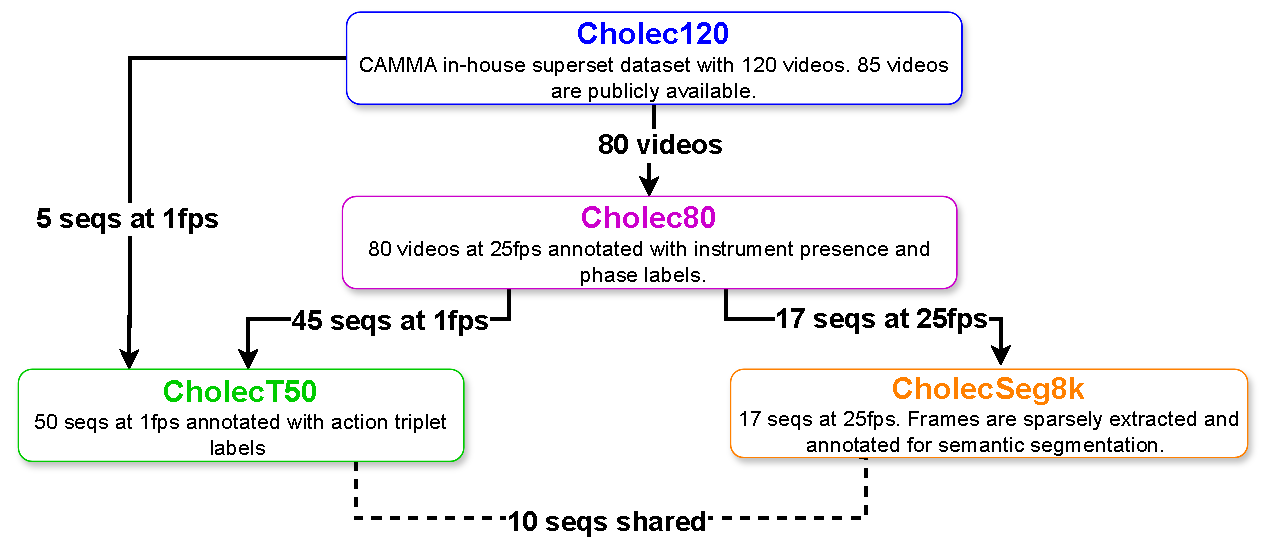
\includegraphics[width=\linewidth]{imgs/cholec_dataset_relationships.pdf}
\caption{CholecInstanceSeg contains frames extracted from CholecT50, CholecSeg8k, and Cholec80. These three datasets are sub-datasets of the CAMMA in-house dataset called Cholec120. There are also some shared image sequences (referred to as \emph{seqs} in the figure for brevity) between CholecT50 and CholecSeg8k.}
\label{fig:cholec_dataset_relationships}
\end{figure}


\subsubsection*{CholecSeg8k}
CholecSeg8k comprises 8,080 laparoscopic cholecystectomy image frames extracted from 17 surgical procedure video clips within the Cholec80 dataset. This dataset provides 80 consecutive images sparsely annotated for semantic segmentation (but not instance segmentation).
To enhance CholecSeg8k, instance IDs are required for the existing semantic segmentation labels. As CholecSeg8k already contains semantic segmentation labels, it serves as a good starting point for further annotation. However, it is important to note that CholecSeg8k includes only two tool classes: Grasper and Hook, which is fewer than the number of tool classes  in the parent datasets.

\subsubsection*{CholecT50}
CholecT50 is a publicly available dataset comprising 50 real-world videos of laparoscopic cholecystectomy surgeries. This dataset integrates 45 videos from the Cholec80 dataset along with 5 additional videos from the in-house Cholec120 dataset. 
The image sequences in CholecT50 are extracted at a rate of 1 frame per second (fps). Each frame in CholecT50 is annotated with fine-grained tool-tissue interaction labels, specifying the \texttt{<instrument, action, target>}. Although CholecSeg8k and CholecT50 share 10 image sequences, we confirmed that the video extraction methods used for these datasets are different. We checked the similarity between extracted frames in the shared sequences from both datasets and found no exact matches.

The CholecT50 dataset consists of 100.9k frames distributed across 50 image sequences. Given the high cost of annotating every single frame, we adopted a strategy to balance thoroughness and feasibility. Consequently, we divided CholecT50 into two partitions:
%
\begin{enumerate}
    \item CholecT50-full: This partition was chosen to feature comprehensive annotations, including instance IDs and segmentation masks for every frame in the image sequence. This thorough annotation provides detailed data for in-depth analysis and model training, allowing for the exploration of ideas like video segmentation.
    \item CholecT50-sparse: In this partition, annotations are provided sparsely in time, yet they cover the entire sequence. This approach reduces annotation costs while still offering valuable insights into the location and identification of tools for each sequence. We sample one in every 30 frames ($\frac{1}{30}$ fps) and add more frames if the resulting sample contains fewer than 50 frames per sequence.
\end{enumerate}


\subsubsection*{Cholec80}
Cholec80 comprises 80 videos of cholecystectomy surgeries. It is labelled with phase information at 25 fps and tool presence annotations at 1 fps. The tool annotations include instruments where at least half of the tool-tip is visible. There are six tools available in the provided tool presence annotations.

Given the overlap between Cholec80, CholecSeg8k, and CholecT50, we focus on annotating the 28 videos in Cholec80 that are not present in CholecSeg8k and CholecT50. We extract frames from these 28 videos at a rate of $\frac{1}{30}$ fps and provide annotations for these frames. 
To maintain consistency with the extraction protocol of CholecT50 and CholecSeg8k, we blacked out frames that showed the exterior of the body via the laparoscope. Additionally, if the resulting sample contained fewer than 50 frames per sequence, more frames were included to ensure adequate coverage.

\subsubsection*{Summary of CholecInstanceSeg Partitions}
CholecInstanceSeg, which contains 41.9k frames from 85 unique image sequences, can be partitioned into four distinct sections based on the data source: Instance-CholecSeg8k, Instance-CholecT50-full, Instance-CholecT50-sparse, and Instance-Cholec80-sparse. \robustrevref{2}{1}\revnew{Our process for selecting the frames and sequences for each partition is as follows:}
%
%
\begin{enumerate}
    \item Instance-CholecSeg8k: \revmod{We selected} all the 8,080 frames from all the 17 sequences provided in CholecSeg8k, we utilized all the images in CholecSeg8k.
    \item Instance-CholecT50-full: \revmod{We randomly selected}  15 sequences within CholecT50 (CholecT50-full), we utilized all frames provided by CholecT50 for these \revnew{15} sequences \revnew{- 28,317 frames}.
    \item Instance-CholecT50-sparse: For the remaining 35\revnew{(50-15)} sequences in CholecT50(CholecT50-sparse), we sampled these sequences by selecting one frame out of every 30 frames ($\frac{1}{30}$ fps), ensuring a minimum of 50 frames in each sequence \revnew{- 2,681 frames} . 
    \item Instance-Cholec80-sparse: \revmod{After selecting sequences for Instance-CholecSeg8k, Instance-CholecT50 (both full and sparse),} there remained 28 videos from Cholec80, which are not included in CholecT50 and CholecSeg8k, and these videos were sampled at $\frac{1}{30}$ fps, ensuring a minimum of 50 frames in each sequence \revnew{- 2,855 frames} . 
\end{enumerate}
%
A visual representation of dataset partitions in CholecInstanceSeg can be seen in \figref{fig:our_dataset}.

\robustrevref{1}{6}\revnew{The differences in frame rates for each dataset partition reflect both the design of the parent datasets -- Cholec80 provides videos at 25fps which we then extract at 1fps and CholecT50 provides image sequences at 1fps directly -- and practical considerations for annotating instance segmentation on a large number of frames. Annotating every sequence densely at 1fps is prohibitively expensive. Thus, we adopted a mixed approach, converting existing semantic segmentation to instance segmentation, annotating some sequences \emph{fully} (using all frames available from the parent datasets), and others sparsely (sampling frames at reduced frame rates of $\frac{1}{30}$ fps). This approach allows us to balance annotation density and dataset diversity, ensuring coverage of both densely annotated sequences and a wider range of surgical scenes.}


\robustrevref{2}{1}\revnew{ \figref{fig:recommended_dataset_splits} presents the exact sequences in each partition, represented as VID-XX, where XX is the sequence number. 
}










\begin{figure}[ht]
  \centering
  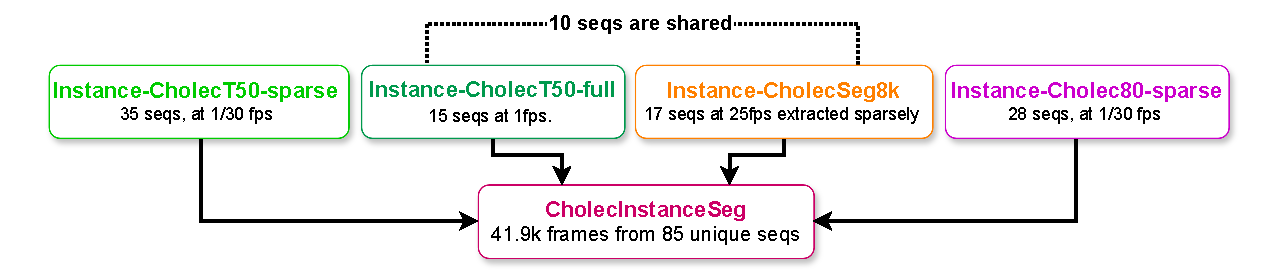
\includegraphics[width=\linewidth]{imgs/cholec_instance_seg_map.pdf}
   \caption{CholecInstanceSeg is composed of frames from four dataset partitions: Instance-CholecT50-sparse, Instance-CholecT50-full, Instance-CholecSeg8k, and Instance-Cholec80-sparse. The diagram illustrates the number of image sequences (denoted \emph{seqs} in the figure for brevity) and extraction rates for each partition. Note that 10 sequences are shared between Instance-CholecT50-full and Instance-CholecSeg8k.}
   \label{fig:our_dataset} 
\end{figure}

\subsection*{The Labelling Protocol}
To facilitate the creation of a high-quality instance segmentation dataset for laparoscopic cholecystectomy videos, we established specific rules to ensure accurate and consistent identification and segmentation of surgical instruments. These rules are discussed under three main topics: Tool Categories, Annotation Scope, and Annotation Guidelines.

\subsubsection*{Tool Categories}
In this section, we detail the tool categories selected for annotation and discuss the objects that were deliberately excluded, along with the rationale for these decisions.

We identified seven tool categories for annotation based on our observations from the extracted CholecInstanceSeg sequences:
\begin{enumerate}
    \item Grasper: Standard grasper used for holding tissues.
    \item Bipolar: Bipolar grasper used for grasping and coagulation.
    \item Hook: Monopolar hook used for dissection and coagulation.
    \item Clipper: Clip applier used for applying clips.
    \item Scissors: Monopolar scissors used for cutting tissues.
    \item Irrigator: Suction/irrigation device used for fluid management.
    \item Snare: Laparoscopic snare used for ligation of tissues.
\end{enumerate}

The inclusion of the snare category deviates from the standard six categories (grasper, bipolar, hook, clipper, scissors, irrigator) defined by Cholec80 and CholecT50. We determined that the snare's distinct visual characteristics and unique functionality warranted its classification as a separate tool category. 

\revdel{A visual representation of these tool categories is shown in \figref{fig:tools}}

% \begin{figure}[ht]
%   \centering
%    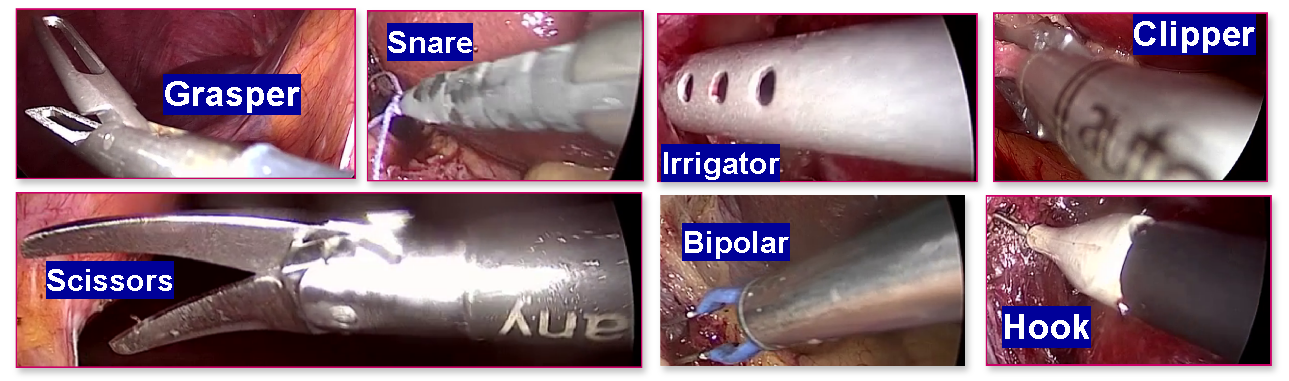
\includegraphics[width=\linewidth]{imgs/tools_cholecinstanceseg.pdf}
%    \caption{Visual representation of the tool categories used in the CholecInstanceSeg dataset. Each image shows a different tool: Grasper, Snare, Irrigator, Clipper, Scissors, Bipolar, and Hook.}
%    \label{fig:tools}
% \end{figure}


\subsubsection*{Annotation Scope}
The annotation scope defines the entities included and excluded to maintain a focused and high-quality dataset. While we annotated all laparoscopic tools,  some objects used in conjunction with these tools were excluded to streamline the annotation process:
%
\begin{itemize}
    \item Excluded Entities: Individual clips from the clipper, surgical needles, surgical sutures, the specimen bag, the camera port, and gauze.
    \item Instrument Ports: We did not annotate the instrument port when no instrument extended from it. However, when an instrument was seen extending from the port, we annotated the instrument port as part of the instrument. This approach aligns with the CholecSeg8k annotation style and addresses the difficulty of distinguishing the exact point where the port ends and the instrument begins. 
    
    \revdel{A clear visual representation of this unique situation with the instrument port can be seen in \figref{fig:instrument_port}}
\end{itemize}

% \begin{figure}[ht]
% \centering
% 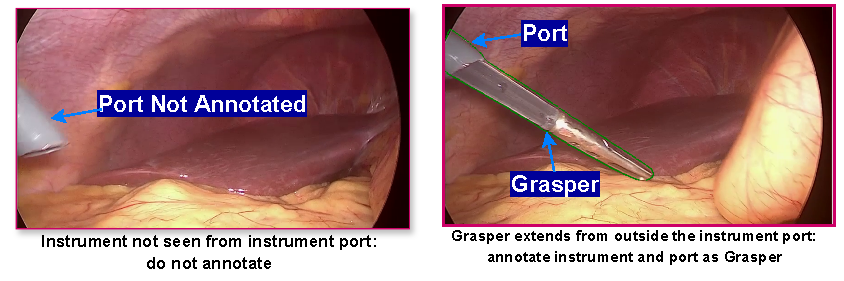
\includegraphics[width=\linewidth]{imgs/instrument_port_interaction.pdf}
% \caption{A visual representation of the unique annotation situation with the instrument port. On the left, no annotation is made when the instrument is not seen extending from the port. On the right, the instrument and the port are annotated as a single entity when the instrument extends from the port.}
% \label{fig:instrument_port}
% \end{figure}

\subsubsection*{Annotation Guidelines}
Our annotation guidelines ensure consistency and accuracy in the labelling process. These guidelines cover various scenarios and provide specific instructions for annotators:
%
% \begin{figure}[ht]
% \centering
% 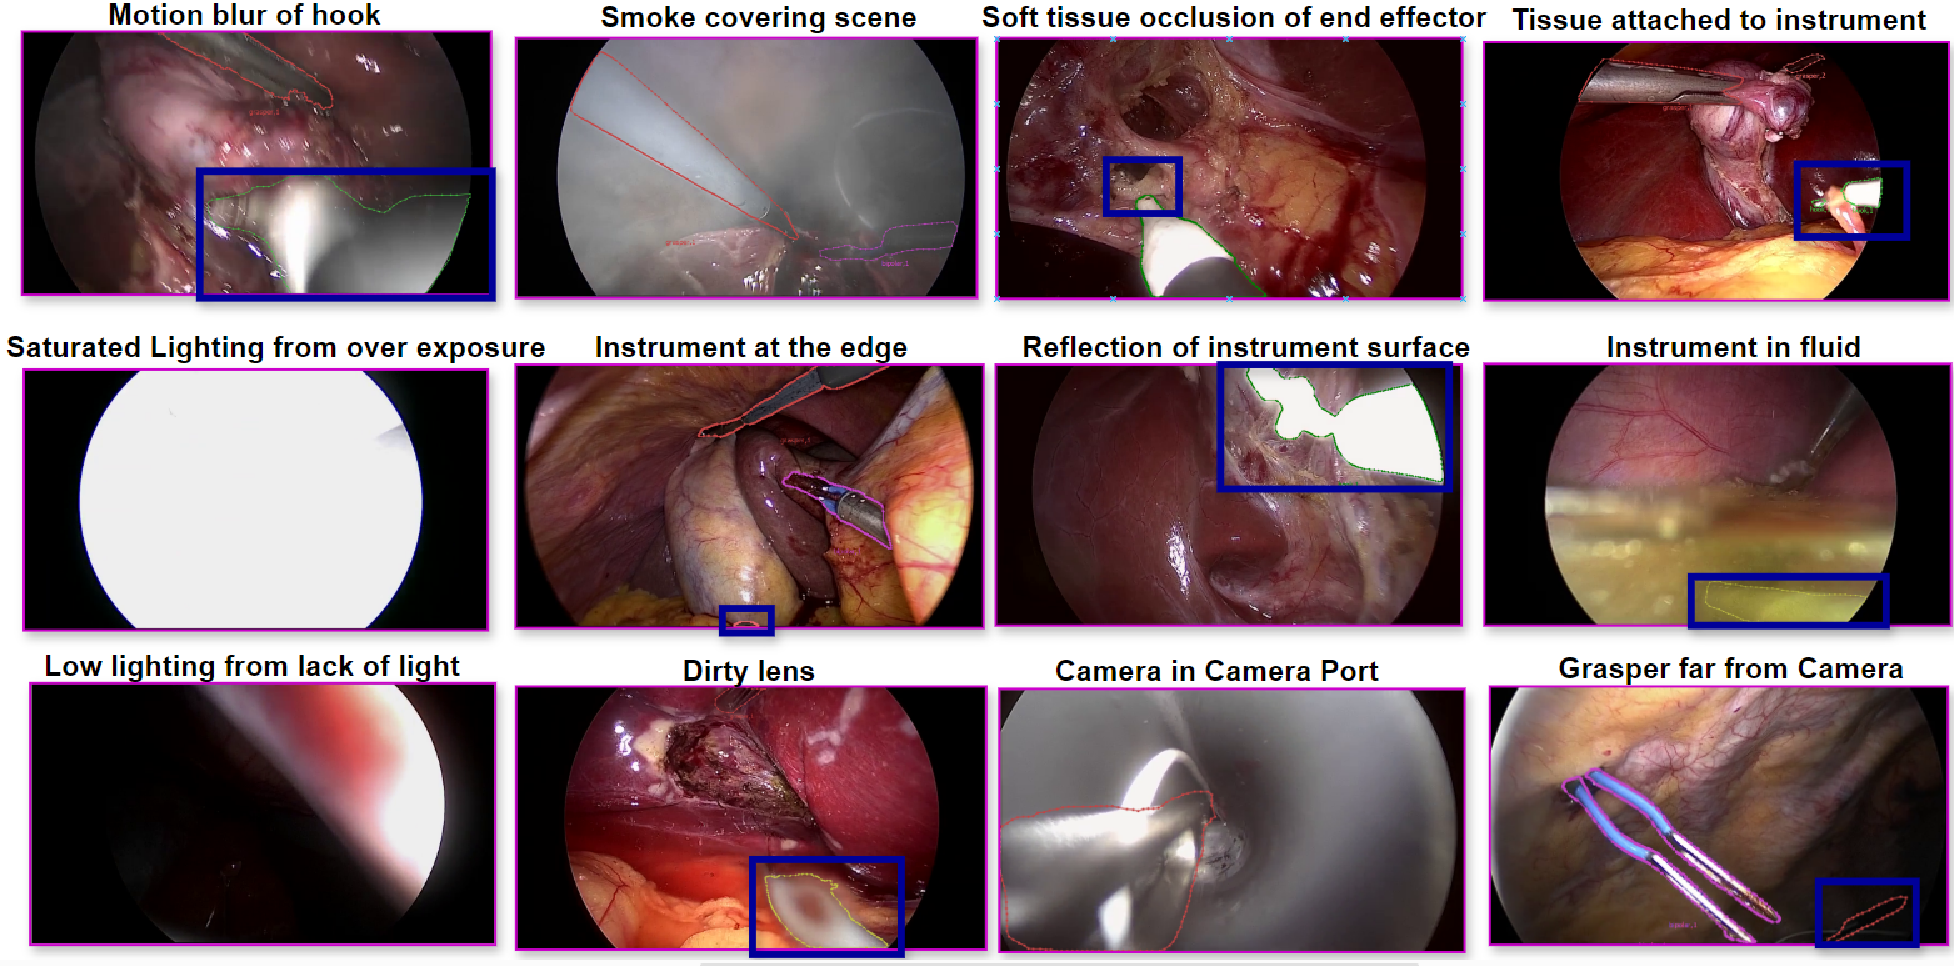
\includegraphics[width=\linewidth]{imgs/all_hard_cases.pdf}
% \caption{Visual representation of challenging annotation scenarios. Each image highlights a specific hard case: motion blur, smoke, soft tissue occlusion, tissue attachment, saturated lighting, instrument at the edge, reflection, instrument in fluid, low lighting, dirty lens, camera in port, and instrument far from the camera. \robustrevref{1}{14}\revnew{The tool instance segmentation annotations are provided as coloured outlines around each tool.}}
% \label{fig:hard_cases}
% \end{figure}
%
%
\begin{itemize}
    \item Annotation Quality: We aimed to annotate every visible instrument while maintaining high segmentation quality. Although achieving pixel-perfect annotation for every instance was impractical due to time and budget constraints, we allowed minor imperfections in instrument boundaries, provided that the fundamental characteristics of the instrument and its end-effectors were accurately outlined. Holes within instruments were considered integral parts of the instrument itself, following the standard annotation conventions in popular tool segmentation datasets like EndoVis2017 \cite{endovis2017_cis} and EndoVis2018 \cite{endovis2018_cis}.
    \item Annotation of Hard Cases:  CholecInstanceSeg captures routine surgical procedures, numerous challenging scenarios were encountered. We accounted for twelve specific situations: motion blur, presence of smoke, occlusion by soft transparent tissues or blood, tissues attached to instruments, instruments at the edge of the frame, instruments far from the camera, light reflection, low lighting conditions, bright lighting conditions, lens dirtiness, camera in camera port, and instruments in liquid.
    Specialized instructions and examples were provided to annotators, including checking neighbouring frames for clarification, utilizing the expected shape of the instrument when in doubt, annotating as much of the instrument as possible, and annotating even under low visibility conditions. 
    \revdel{A visual representation of these hard cases can be seen in \figref{fig:hard_cases}.  More detailed information about specialized instructions given to annotators for hard cases is added as supplementary material for this manuscript.} 
\end{itemize}




\subsection*{Annotation Tool and Techniques} \label{sec:annotation_methods}
To provide annotations for CholecInstanceSeg, we needed an annotation tool for performing manual annotations, a method to convert existing semantic segmentation to instance segmentation, and a way to efficiently label a large number of images. This section discusses how we addressed these needs: the annotation tool, converting semantic segmentation to instance segmentation, and semi-automatic annotation.

\subsubsection*{Annotation Tool}\label{sec:annotation_tool}
Data labelling was primarily executed using a minimally customized version of the \href{https://github.com/haochenheheda/segment-anything-annotator}{Segment Anything Annotator tool} \cite{wangsupplementary}, which is open-source software based on the \href{https://github.com/labelmeai/labelme}{LabelMe} annotation project \cite{wada2016labelme}. This tool integrates instrument segmentation functionalities and interactive segmentation capabilities, leveraging the Segment Anything Model (SAM) \cite{kirillov2023segment_cis}. Our customizations included enhancements for navigation, reduction in the size of annotation label files, and the addition of a quality control mode. The customized version is available \href{https://github.com/labdeeman7/my_samannotator}{on github}.

We predominantly utilized point-based SAM prompts for efficient and quick interactive annotation. However, point-prompt-based interactive segmentation often encounters challenges in complex scenarios, such as when instruments and surrounding backgrounds are similar in color, low lighting, glare, blurs, dirty lenses, reflections, and the presence of smoke. In such instances, manual annotation can also be performed using the same tool. Further discussion of challenging scenarios is provided in a later section.

\subsubsection*{Converting Semantic to Instance Segmentation} \label{sec:semantic_to_instance}
One of our data sources, CholecSeg8k, already had semantic segmentation labels. However, we aimed to assign instance IDs to distinguish each instrument instance within an image. To add instance labels and convert existing semantic segmentation labels to instance segmentation, we followed two main steps:

\begin{enumerate}
    \item \textbf{Class-Aware Connected Component Analysis}: We employed connected component analysis for each class separately to identify and segregate different instances within the frames. This technique effectively assigned instance IDs to instruments from different classes and correctly distinguished instances of instruments belonging to the same class that do not overlap in pixel space.
    \item \textbf{Identifying and Addressing Failure Cases}: Class-aware connected component analysis encountered several challenges. A total of 892 frames with these issues were carefully identified and documented. To rectify these problems, we developed and applied several pipelines:
        \begin{enumerate}
            \item \textbf{Occlusions}: When pixels of the same instrument are not connected, class-aware connected component analysis assigns multiple instance IDs to a single instrument. This issue, mainly caused by occlusions at the frame's edge or by tissues, was addressed by combining multiple instances that were actually the same using a Python pipeline.
            \item \textbf{Overlap}: A single instance ID was assigned to different instances of the same instrument class that overlapped in pixel space. We reannotated these frames using our annotation tool.
            \item \textbf{Dataset Noise}: Stray erroneous pixels, incorrect instrument class labels, and missing instrument annotations led to incorrect instance ID assignments. We built pipelines to remove instances caused by dataset noise and correct class labels. Missing instruments were also annotated as required.
        \end{enumerate}
\end{enumerate}

\subsubsection*{Semi-Automatic Annotation}
For the CholecT50-full dataset, which requires annotations for full sequences (nearly 30,000 frames from 15 sequences extracted at 1 fps), we opted for a semi-automatic approach with a human-in-the-loop, utilizing a deep learning model to assist in producing instance segmentation annotations.

\begin{enumerate}
    \item Initial Annotation: We began with initial annotations from the Instance-CholecSeg8k dataset. Since CholecSeg8k only contains two tool categories (Grasper and Hook), which is fewer than the seven tool categories identified for annotation, we performed additional annotations using the annotation tool. We focused on images that included the new instruments. The combined dataset of Instance-CholecSeg8k and these initial annotations provided a foundation to start the semi-automatic pipeline for generating labels.
    \item Model Training:  A deep neural network, the Real-Time Models for Object Detection and Instance Segmentation Large (RTMDet-Ins-l) \cite{lyu2022rtmdet}, was trained using the available annotated datasets (Instance-CholecSeg8k and Instance-CholecT50-sparse). 
    \item Annotation Proposal Generation: Leveraging the trained model, we generated annotations for a larger portion of the unannotated data.
    \item Annotation review and correction: Human annotators reviewed the model-generated annotations and corrected any errors or inaccuracies, ensuring the quality and accuracy of the annotations. \robustrevref{1}{13}\revnew{Minor errors were corrected with the capabilities of the LabelMe labeling tool, while major errors requiring new annotations utilized the point-prompt method of the SAM model.}
    \item Augment training dataset:  The machine learning model was retrained using the expanded training dataset, incorporating the corrected annotations. This iterative process enhanced the model's performance. 
    The model was trained twice: initially, with an annotation set of approximately 11k images and their corresponding labels. The trained models was used to generate labels for about 10k images. Human annotators corrected labels for 5k of these images. The model was then retrained with 21k images, generating labels for another 17k images, with labels for 4k images requiring human annotators for correction.
\end{enumerate}
%
A visual representation of our semi-automatic approach to annotation can be seen in \figref{fig:annotation_pipeline}.

\begin{figure}[ht]
  \centering
   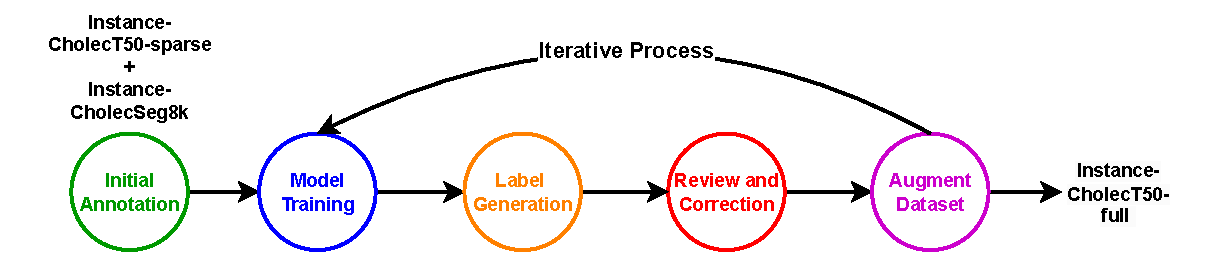
\includegraphics[width=0.9\linewidth]{imgs/train-retrain-annotate.pdf}
   \caption{Semi-automatic annotation pipeline. The process begins with initial annotations using Instance-CholecT50-sparse and Instance-CholecSeg8k, followed by model training. The trained model generates labels, which are then reviewed and corrected by human annotators. The corrected annotations augment the training dataset, iterating through the cycle until the final Instance-CholecT50-full dataset is produced.}
   \label{fig:annotation_pipeline}
\end{figure}

\subsection*{Annotation Workflow and Procedures}
This section provides an overview of the step-by-step procedure used to create the CholecInstanceSeg dataset, along with detailed insights into the human effort involved in the annotation process. We organize the discussion into two main topics: the step-by-step procedure, and Annotators.

\subsubsection*{Step-by-Step Procedure}

\begin{enumerate}
    \item Annotation of Instance-CholecSeg8k (2 weeks): Converted the CholecSeg8k dataset, which initially contained semantic segmentation labels, into Instance-CholecSeg8k with instance IDs. Quality checks were performed to ensure accuracy. This dataset partition only had two classes and lacked many challenging scenarios present in other datasets.
    \item Creating the Labelling Protocol (3 weeks): Extensive discussions among the annotation team addressed the challenges encountered during the initial annotation attempts of the Instance-CholecT50-sparse partition. These discussions led to the development of a comprehensive labelling protocol to handle hard cases and unique scenarios effectively and consistently.
    \item Annotation of Instance-CholecT50-Sparse (3 weeks): Annotated the Instance-CholecT50 dataset partition using the annotation tool. This occurred in tandem with the creation of the labelling protocol. Quality checks ensured annotations were accurate and consistent with the newly established guidelines.
    \item Annotation of Instance-CholecT50-Full (3 weeks): Using Instance-CholecT50-Sparse and Instance-CholecSeg8k as initial annotations, we employed a semi-automatic pipeline to generate the Instance-CholecT50-Full dataset. This process included iterative model training and corrections to enhance annotation quality.
    \item Annotation of Instance-Cholec80 (1 week): To ensure comprehensive coverage and enhanced diversity for CholecInstanceSeg, we utilized the annotation tool to manually annotate the Instance-Cholec80 partition.
    \item Final Quality Control (2 weeks): Quality control was conducted after the creation of each dataset and again upon finalizing CholecInstanceSeg. This process included several steps to ensure accuracy and consistency. Initially, we performed manual quality control, manually reviewing each image to ensure correct annotations. A second annotator then reviewed a subset of CholecInstanceSeg and performed additional corrections.

    We also leveraged specific properties of CholecInstanceSeg and its relationships with other datasets to enhance quality control. For instance, we used existing tool presence labels from related datasets for cross-validation. Detailed steps for quality control, utilizing these properties and external dataset labels, are extensively discussed in the \hyperlink{sec:quality_control}{quality control section}.
\end{enumerate}

\subsubsection*{Annotators}
The annotation process for creating the CholecInstanceSeg dataset involved a primary annotator responsible for the majority of the annotation tasks and quality control. A secondary annotator, with greater experience and medical qualifications, assisted with annotation and quality control. Both annotators were supported by an expert team to ensure accuracy and consistency in the annotations.







